%=========================================================================
% sec-intro
%=========================================================================

\section{Introduction and Problem Statement}
\label{sec-intro}

\begin{figure}[b]
  \begin{minipage}[b]{0.42\tw}
    %=========================================================================
% fig-intro-overview
%=========================================================================

%\begin{figure}

  \centering
  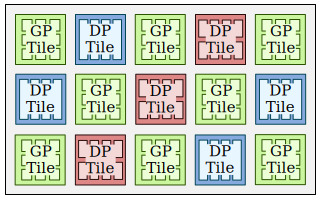
\includegraphics[width=0.85\tw]{intro-overview.svg.pdf}

  \caption{\textbf{Example of Fine-Grain Heterogeneous Architectures --}
    A sea of lightweight compute tiles composed of both general-purpose
    tiles (GP tiles) and data-parallel accelerators specialized for
    exploiting different forms of data parallelism (DP tiles).}

  \label{fig-intro-overview}

%\end{figure}

  \end{minipage}%
  \hfill%
  \begin{minipage}[b]{0.56\tw}
    %=========================================================================
% fig-intro-vision
%=========================================================================

%\begin{figure}

  \centering
  \includegraphics[width=\tw]{intro-vision.svg.pdf}

  \caption{\textbf{XPC Architecture Overview --} XPC applications use an
    XPC parallel programming library to expose fine-grain parallel tasks.
    A software runtime is used to facilitate adaptive task distribution
    across XPC tiles based on statistics collected during profiling. The
    heterogeneous XPC tiles are specialized for various forms of
    parallelism, but all XPC tiles have a common ISA.}

  \label{fig-intro-vision}

%\end{figure}

  \end{minipage}
\end{figure}

Microprocessor design has reached the limits of improving performance and
energy efficiency by scaling the number of general-purpose cores on a
chip. Instead, computer architects are increasingly using a heterogeneous
mix of general-purpose cores and data-parallel accelerators to exploit
the ubiquitous data parallelism present in modern applications such as
graphics rendering, computer vision, audio processing, graph processing,
physical simulation, big data analytics, and machine learning. Recent
examples include Intel
Haswell~\cite{hammarlund-intel-haswell-ieeemicro2014}, AMD
Kabini~\cite{bouvier-amd-kabini-ieeemicro2014}, and NVIDIA Tegra
4~\cite{krewell-nvidia-tegra4-mpr2013}, which integrate general-purpose
multicores with programmable graphics processing units (GPUs) at a coarse
granularity. While this is a promising first step, coarse-grain
integration makes it difficult to exploit fine-grain parallelism and/or
to rapidly migrate applications between general-purpose processors and
GPUs. I am interested in exploring future systems that use a
\emph{fine-grain intermingling} of many lightweight general-purpose cores
and data-parallel accelerators unified through a common instruction set
with support for \emph{seamless adaptive execution} of parallel tasks as
shown in Figure~\ref{fig-intro-overview}.
These accelerators would be specialized for a broad range of
\emph{amorphous data parallelism}, a generalized form of data parallelism
where tasks are generated dynamically and can modify the underlying data
structures in unpredictable ways potentially creating inter-task
conflicts~\cite{pingali-tao-pldi2011}. Mapping such applications to
current data-parallel accelerators can be difficult and usually requires
aggressive software
optimizations~\cite{luo-gpu-bfs-dac2010,harish-large-graph-gpu-hipc2007,
  hong-cuda-max-warp-ppopp2011,nasre-data-vs-topo-ipdps2013,
  nasre-morph-ppopp2013,mendez-optimizations-amorphous-ppopp2010,
  mendez-gpu-pta-ppopp2012}.
\BF{This proposal outlines the explicit-parallel-call (XPC) architecture,
  a novel fine-grain heterogeneous architecture based on the concept of
  explicitly encoding parallel tasks as parallel function calls in the
  software/hardware interface.} Figure~\ref{fig-intro-vision} highlights
the vertically integrated approach that will be used to explore both
software and hardware techniques for \emph{exposing}, \emph{executing},
and \emph{scheduling} fine-grain parallel tasks.

